\documentclass{sig-alternate-ipsn13}

\usepackage{array}
\usepackage{url}
\usepackage{cite}
\usepackage{subfigure}
\usepackage{float}
\usepackage{pdfpages}

%%%%%%%% Package for source-code listing %%%%%%%%%%%%
\usepackage{textcomp,listings}
\definecolor{javared}{rgb}{0.6,0,0} % for strings
\definecolor{javagreen}{rgb}{0.25,0.5,0.35} % comments
\definecolor{javapurple}{rgb}{0.5,0,0.35} % keywords 

\lstset{
	language=Java,
	frame=lines,
	captionpos=b,
	basicstyle=\color{blue!30!black!90!green} \ttfamily, % print whole listing small
	keywordstyle=\color{javapurple}\bfseries,%\underbar, underlined bold black keywords
	identifierstyle=, % nothing happens
	commentstyle=\color{javagreen}, % white comments
	stringstyle=\color{javared}, % type for strings
	showstringspaces=false, % no special string spaces
	mathescape=true, % allow math typesetting in listings
	upquote=true,
}
%%%%%%%% Package for source-code listing %%%%%%%%%%%%


%%%%%%%% Packages for drawing diagrams %%%%%%%%%%%%%%%
\usepackage{tikz,ifthen}
\usetikzlibrary{arrows,
	%trees,backgrounds,automata,shapes,snakes,plotmarks,fit,calc,positioning,shadows
}
\tikzstyle{block}=[rectangle, draw, thin, inner sep=3pt, text centered, 
%drop shadow, 
fill=orange!20!yellow!20] 
\tikzstyle{pre}=[<-,shorten <=1pt,>=stealth']
\tikzstyle{post}=[->,shorten >=1pt,>=stealth'] 
\tikzstyle{bi}=[<->,shorten >=1pt,shorten <=1pt,>=stealth'] 
\tikzstyle{every initial by arrow}=[initial text={},initial distance=1em,post]
\tikzstyle{every state}=[minimum size=0.4cm,drop shadow,fill=orange!20!yellow!20]
\tikzstyle{transition}= [post,shorten >=1pt,node distance=2cm, inner sep=2pt,bend angle=20]
\tikzstyle{box}=[rectangle,draw=black, thick, inner sep=3pt, text centered]
%%%%%%%% Package for drawing diagrams %%%%%%%%%%%%%%%

\newcommand\esti{{\lstinline'estimate'}}
\newcommand\simu{{\lstinline'simulate'}}
\renewcommand\j[1]{{\lstinline'#1'}}

\usepackage[english]{babel}
\usepackage{graphicx}
\usepackage{amssymb}
%\usepackage{MnSymbol}

\RequirePackage{pgf,pgffor}


\usepackage[mathcal]{euscript}
%%% END LaTeX-Packages ----------------------------------


\usepackage{setspace}
\newcommand\tuple[1]{\langle #1 \rangle}

\newcommand\sSF[1]{$\Diamond$\footnote{SF: \sout{#1}}}
\newcommand\sIL[1]{$\Diamond$\footnote{IL: \sout{#1}}}
\newcommand\sMA[1]{$\Diamond$\footnote{MA: \sout{#1}}}
\newcommand\sGW[1]{$\Diamond$\footnote{GW: \sout{#1}}}


\newcommand\SF[1]{$\bigstar$\footnote{SF: #1}}
\newcommand\IL[1]{$\bigstar$\footnote{IL: #1}}
\newcommand\MA[1]{$\bigstar$\footnote{MA: #1}}
\newcommand\GW[1]{$\bigstar$\footnote{GW: #1}}

\newcommand\R{{\mathbb R}}
\newcommand\N{{\mathbb N}}
\newcommand\must{$\mathtt{must}$}
\newcommand\bad{$\mathtt{bad}$}
\newcommand\code[1]{{\small \sf #1}}

%%% LaTeX definitions -----------------------------------------
\newtheorem{thm}{Theorem}
\newtheorem{dfn}[thm]{Definition}
\newtheorem{con}[thm]{Construction}
\newtheorem{prop}[thm]{Proposition}
\newtheorem{claim}[thm]{Claim}

\DeclareMathOperator*{\guard}{guard}
\DeclareMathOperator*{\sensor}{sen}
\DeclareMathOperator*{\actuator}{act}

\newcommand{\mathsym}[1]{{}}
\newcommand{\unicode}[1]{{}}

\newcommand{\M}{{\mathcal{M}}}
%%% END own LaTeX definitions ---------------------------


\begin{document}

\title{Reactive Scheduling of Computational \\ Resources in Control Systems}
%
% You need the command \numberofauthors to handle the 'placement
% and alignment' of the authors beneath the title.
%
% For aesthetic reasons, we recommend 'three authors at a time'
% i.e. three 'name/affiliation blocks' be placed beneath the title.
%
% NOTE: You are NOT restricted in how many 'rows' of
% "name/affiliations" may appear. We just ask that you restrict
% the number of 'columns' to three.
%
% Because of the available 'opening page real-estate'
% we ask you to refrain from putting more than six authors
% (two rows with three columns) beneath the article title.
% More than six makes the first-page appear very cluttered indeed.
%
% Use the \alignauthor commands to handle the names
% and affiliations for an 'aesthetic maximum' of six authors.
% Add names, affiliations, addresses for
% the seventh etc. author(s) as the argument for the
% \additionalauthors command.
% These 'additional authors' will be output/set for you
% without further effort on your part as the last section in
% the body of your article BEFORE References or any Appendices.

\numberofauthors{2} %  in this sample file, there are a *total*
% of EIGHT authors. SIX appear on the 'first-page' (for formatting
% reasons) and the remaining two appear in the \additionalauthors section.
%
\author{
% You can go ahead and credit any number of authors here,
% e.g. one 'row of three' or two rows (consisting of one row of three
% and a second row of one, two or three).
%
% The command \alignauthor (no curly braces needed) should
% precede each author name, affiliation/snail-mail address and
% e-mail address. Additionally, tag each line of
% affiliation/address with \affaddr, and tag the
% e-mail address with \email.
%
% 1st. author
    \alignauthor Gera Weiss\\
       \affaddr{Ben-Gurion University}\\
       \affaddr{Beer-Sheva, Israel}\\
       \email{geraw@cs.bgu.ac.il}
% 2th. author
    \alignauthor Hodai Goldman\\
        \affaddr{Ben-Gurion University}\\
        \affaddr{Beer-Sheva, Israel}\\
        \email{hodaig@cs.bgu.ac.il}
}

\maketitle
\begin{abstract}

\end{abstract}

\section{Introduction}
Cyber-physical systems (CPS) technologies of integrating software and control are at the heart of many critical applications (c.f.~\cite{lee2008cyber}). 
These technologies aim at handling issues that emerge when the integration of software and hardware brakes the traditional abstraction layers: when researchers and practitioners are required to consider a unified view that includes both software and hardware. An example of such an issue is the challenge of dynamic assignment of computational resources to software based controllers discussed in, e.g.,~\cite{arzen2000introduction,tabuada2007event,weiss2007automata}. While the computation burden required by the control loops can be ignored in many situations, this is not always the case. A main motivating example studied in this paper is vision based control, where computer vision algorithms acquire state information to be used in a feedback loop (c.f.~\cite{das2002vision,shakernia1999landing,Efraim2017}). Unlike conventional sensors such as accelerometers, gyros, compasses, etc., a visual sensor requires significant processing of the acquired image to prepare the state information for feedback. Since typical cyber-physical application, such as robot control, consist of many control loops, responsible for different aspects of the system, that run simultaneously and share the same computational resources, the computer vision algorithms cannot always be invoked in full power. Alternatively, we propose in this paper a mechanism to dynamically trade CPU consumption vs. measurement accuracy so that data acquisition algorithms run in full power only when the control loop requires accurate data. 

A main challenge in forming mechanisms for the integration of software and control lies in the design of efficient interfaces for integrating the engineering diciplines involved (c.f.~\cite{weiss2007automata}). Components with clearly specified APIs, such as Java library classes, allow designers to build
complex systems effectively in many application domains.  The key to such modular development is
that an individual component can be designed, analyzed, and tested without the knowledge of other
components or the underlying computing platform. When the system contains components with
real-time requirements, the notion of an interface must include the requirements regarding
resources, and existing programming languages provide little support for this.  Consequently,
current development of real-time embedded software requires significant low-level manual effort for
debugging and component assembly (cf.  \cite{Lee00,IEEE03,HS06}).  This has motivated many
researchers to develop compositional approaches and interface notions for real-time scheduling (cf.
\cite{RS01,dH01,MF01,CAHS03,SL08,SLBS04,TWS06,DBLP:conf/lctrts/AuerbachBIKRRT07}).


In this paper we present an approach, a proof-of-concept tool, and a case-study in scheduling computations in embedded control systems. Our approach is based on the automata based scheduling approach, suggested in~\cite{WA07,RTComposer,AW08}, where automata are proposed as interfaces that allow the dynamicity and efficiency of desktop operating systems with the predictability of real-time operating systems. The approach allows for components to specify the CPU resources that they need in a way that gives an application agnostic scheduler the freedom to choose schedules at run-time such that the needs of all the components are met, even of components that were added only at run-time.  The main contributions of this paper relative to the earlier work in this direction is:
(1) We propose an extension of the automata based scheduling frame work that allows to direct the schedule based on the state of the controllers; (2) We propose a technique, based on the theory of Kalman Filters, for designing reactively scheduled controllers; (3) We report on our experience with improving the performance of real-time a vision-based control system (a quadrotor that stabilizes itself in front of a window).

\section{Automata Based Reactive Scheduler}
\label{sec:architecture}

As proposed in earlier work on automata based scheduling (cf.~\cite{WA07,RTComposer,AW08}) we aim at a development process where a system is built as a composition of a set of components where each component is a class in, say C++, accompanied with an automaton. Our addition here is that we allow the automata to be guarded, i.e., the automaton acts as a specification of a reactive system that tells the scheduler which functions of a component it may run in each slot depending on the dynamic state of the controllers.

For scheduling tasks within a slot, we adopt the Logical Execution Time (LET)
abstraction~\cite{DBLP:journals/pieee/HenzingerHK03} that allows deterministic
external interface even when the underlying physical execution layer introduces
bounded non-determinism.

The relation between logical and physical task execution is depicted Figure~\ref{fig:LET} (adopted
from~\cite{DBLP:conf/lctrts/FarcasFPT05}). The diagram depicts an execution of one task in one
logical execution slot.  Logically, the task is released at the beginning of the slot and terminates
at the end of it, i.e., the task processes the inputs captured at the release time and its output
are only made available to the outside world at the logical termination time. The actual execution,
as shown in the figure, may start and finish anywhere in the logical execution slot and the
execution may be interrupted by higher priority tasks. However, the external interface remains
deterministic provided only that all tasks always finish within logical execution slots.


%%%%%%%%%%%%%%%%%%%%%  LET %%%%%%%%%%%%%%%%%%%%%%%%%%%%%%%

\begin{figure}[htb]
	\centering
	
	\def\h{.7cm}
	\def\w{5.5cm}

	\begin{tikzpicture}[minimum height=\h,scale=0.8, every node/.style={scale=0.8}]      
	\node [block,minimum width=\w] (TI) {Task Invocation};
	\node [matrix] at (-.1cm,-\h) {\node [block] {running}; & \node [block,minimum width=.7cm,fill=yellow!10] {waiting}; & \node [block] {running}; \\}; 
	
	\draw [post] (-\w/2,1.2cm) -- (-\w/2,\h/2);
	\node at (-\w/2,1.4cm) {\lstinline!readInputs!};
	
	\draw [pre] (\w/2,1.2cm) -- (\w/2,\h/2);
	\node at (\w/2,1.4cm) {\lstinline!writeOutputs!};
	
	\draw [bi] (-\w/2,\h/4 + .5cm) -- node [above] {Logical Execution Slot} (\w/2,\h/4 + .5cm);
	
	\draw [post,thick] (-\w/2-1cm,-\h/2) -- node [above,at end] {Time}  node [above, at start] {Logical}  node [below, at start] {Actual}  (\w/2+.7cm,-\h/2);
	\end{tikzpicture}
	
	\caption{Execution of a task in an execution slot.}
	\label{fig:LET}
\end{figure}


Diverging from the way LET is applied in other
architectures~(c.f.~\cite{DBLP:journals/pieee/HenzingerHK03,DBLP:conf/lctrts/AuerbachBIKRRT07}),
our architecture executes a dynamic assignment of tasks to logical execution slots.  Specifically, the set
of tasks that run in each logical execution slot is chosen from the composition of all resource
specifications of the components. The scheduler has a complete view of resource requirements and can allocate them accordingly. For example, the system we
can react to an increased need of CPU of one of the components by reducing the non real-time computations.

%To implement the above semantics, we propose a scheduling mechanism consisting of
%a macro (intra-slot) scheduler and a micro (inter-slot) scheduler, as follows. 
%The micro scheduler is the built-in
%scheduler provided by the Java virtual machine (or even a real-time Java virtual machine). We use it to run all tasks,
%including interrupt handlers, controller components and background applications.
%The macro scheduler mediates the execution of the real-time components, as
%follows. At the beginning of every logical execution slot, the macro scheduler
%invokes all \lstinline!readInput! methods and spawns a set of tasks that wrap the
%methods of the real-time components to be executed in that slot. At the end of
%the slot, the macro scheduler invokes all \lstinline!writeOutput! methods.
%
%
%Priorities are assigned as follows. The lowest priority is assigned to the background applications that run only when the real-time threads and the interrupt handlers are
%inactive. The highest priority is given to interrupt handlers and to the macro scheduler which is considered as the highest priority interrupt handler (assuming that
%\lstinline!readInputs! and \lstinline!writeOutputs! are short and deterministic).  The real-time tasks, spawned by the macro scheduler, run in a priority higher than all
%background application and lower than interrupt handlers.
%
%Note that our approach is independent of the algorithm used by the micro scheduler for tasks scheduling, which can be, e.g., Earliest Deadline First (EDF), Least Slack Time (LST), rate Monotonic (RM), Deadline Monotonic (DM) or any scheduling algorithm that allows guarantees of termination of all tasks before the end of each slot. More generally, the interface with the micro-scheduled does not have to be the set of tasks to run in a slot.
%
%A notable advantage of using automata based scheduling is that new components can be added without disturbing the continuous execution of existing ones.  Specifically, when a new component is added, the existing components are assured to continue a schedule which satisfies their scheduling specifications, but possibly not the one that was planned (because the new component may not allow the one that was planned).
%As a simple example, consider the following component $C_1$ depicted in  Listing~\ref{lst:c1}. The methods f1, f2 need to execute cyclically (for all $i=0,1,2,\dots$ and $j=1,2$, the function \lstinline!f$j$! needs to execute in slot $2i+j$).
%Assume that this component is added and scheduled for a while. Later on, anther component $C_2$ depicted in Listing~\ref{lst:c2} is added.
%$C_2$ has two methods g1, g2 that need to execute cyclically too. When the second component is added, the count of the running component should not be disturbed.
%
%%\begin{figure}[h!]
%%\begin{center}
%%\noindent\begin{minipage}{.5\textwidth}
%\begin{lstlisting}[language=java,label=lst:c1,caption=First Component.]
%class C1 implements Component {
%...
%
%@WCET(0.2)
%public void f1() { 
%...  
%} 
%
%@WCET(0.8)
%public void f2() { 
%...  
%} 
%
%}
%\end{lstlisting}
%
%%\end{minipage} \hspace{1cm}
%%\begin{minipage}{.5\textwidth}
%\begin{lstlisting}[label=lst:c2,caption=Second Component.]
%class C2 implements Component {
%...
%
%@WCET(0.3)
%public void g1() { 
%...  
%} 
%
%@WCET(0.1)
%public void g2() { 
%...  
%} 
%
%}
%\end{lstlisting}
%%\end{minipage}
%%\end{center}
%
%
%%\caption[ABCDE]{blaaa}
%%\label{qwert}
%%\end{figure}
%
%%\lstlistoflistings
%%\begin{mycode}
%%\begin{minipage}[t]{0.3\linewidth}
%
%%\begin{lstlisting}[float=htb,linewidth=7cm,caption=First Component.Already scheduled for a while.]
%%class C1 implements Component {
%%  ...
%%
%%  @WCET(0.2)
%%  public void f1() { 
%%    ...  
%%  } 
%%
%%  @WCET(0.8)
%%  public void f2() { 
%%    ...  
%%  } 
%%
%%}
%%\end{lstlisting} 
%
%%\end{minipage}
%%\begin{minipage}[t]{0.3\linewidth}
%%\begin{lstlisting}[float=htb,linewidth=7cm,caption=Second Componenct.]
%
%%class C2 implements Component {
%%  ...
%%
%%  @WCET(0.3)
%%  public void g1() { 
%%    ...  
%%  } 
%%
%%  @WCET(0.1)
%%  public void g2() { 
%%    ...  
%%  } 
%%
%%}
%%\end{lstlisting}
%
%%\end{mycode} 
%%\end{eqnarray*}
%%\end{minipage}
%%%%%%%%%%%%%%%%%%%%%%  code 1 %%%%%%%%%%%%%%%%%%%%%%%%%%%%%%%
%
%In a previous versions (RTComposer), macro-scheduling was done by simulating a random walk over the automaton whose language is the intersection of all the scheduling specification of the components. Note that in case that the existing component runs the $f2$ method (whose WCET is 0.8) within the next slot, the intersection between the languages of these two components is empty, because the new component must start with the method $g1$ whose WCET is 0.3, and $f2$ and $g1$ cannot run together within a slot. Therefore, in the previous version, using intersection lead to incorrect schedule.
%In this paper we propose a new way to dealt with this problem. When the new component is added we play a joining game. Based on the game results we know whether this component can be added now or later, or it cannot be added without disturb the flow of the system. This game is built by the product of the running automata and the scheduling specifications of the new component. For more details, see the implementation part of this paper.
%Game is the tool we use for the admission of the new component. In case that the new component was added, the scheduler needs to assure that the existing components will be scheduled consistently with current state of the running automaton. The new schedule will be this product automaton.
%All the computations of the product automaton and the game are done as non-real-time background computations. Also, the new product automaton should not always start executing form its initial state (as the existing components are not necessarily at their initial state). To account for that, and still provide quick turnover, a hash-table is constructed that maps the states of the running automaton to the sates of the automaton that is going to replace it. Then, when the computation of product automaton is completed, the state of the running automaton is replaced with the corresponding state of the new automaton. Removal of components can done in a similar manner.


%\section{An example driven description of the proposed approach}
\section{A demonstration of the approach in simulation}

Our approach for using automata for scheduling resources in software based controllers is based on the observation that in most systems the computational load is in the implementation of the sensors and of the actuators, not in the implementation of the controllers that usually consist of quick arithmetic manipulation of a small amount of variables. We therefore focus our attention on allowing a trade-off between CPU usage of sensors and actuators and their accuracy. In this paper, as a main motivating example, we focus on the case of visual sensors that employ image processing algorithms.

As said in Section~\ref{sec:architecture}, we propose to implement the resource scheduling decisions using automata that control which procedures are invoked in the control loops. More specifically, for sensors or actuators that require heavy computations, such as vision based sensors, we propose that the software engineers develop several modes of sensing, each consumes a different amount of CPU and provides a different level of accuracy. 

Formally, we assume that the system is given as a Linear Time Invariant system, as depicted in Figure~\ref{fig:simulink}. The inaccuracies of the sensors and of the actuators are modeled as additive Gaussian noise. We assume that each sensor can be operated in a range of modes (more than one), each mode consuming a certain percentage of the CPU and giving a certain variance of the measurement noise.

\begin{figure}%[htbp]
	\centerline{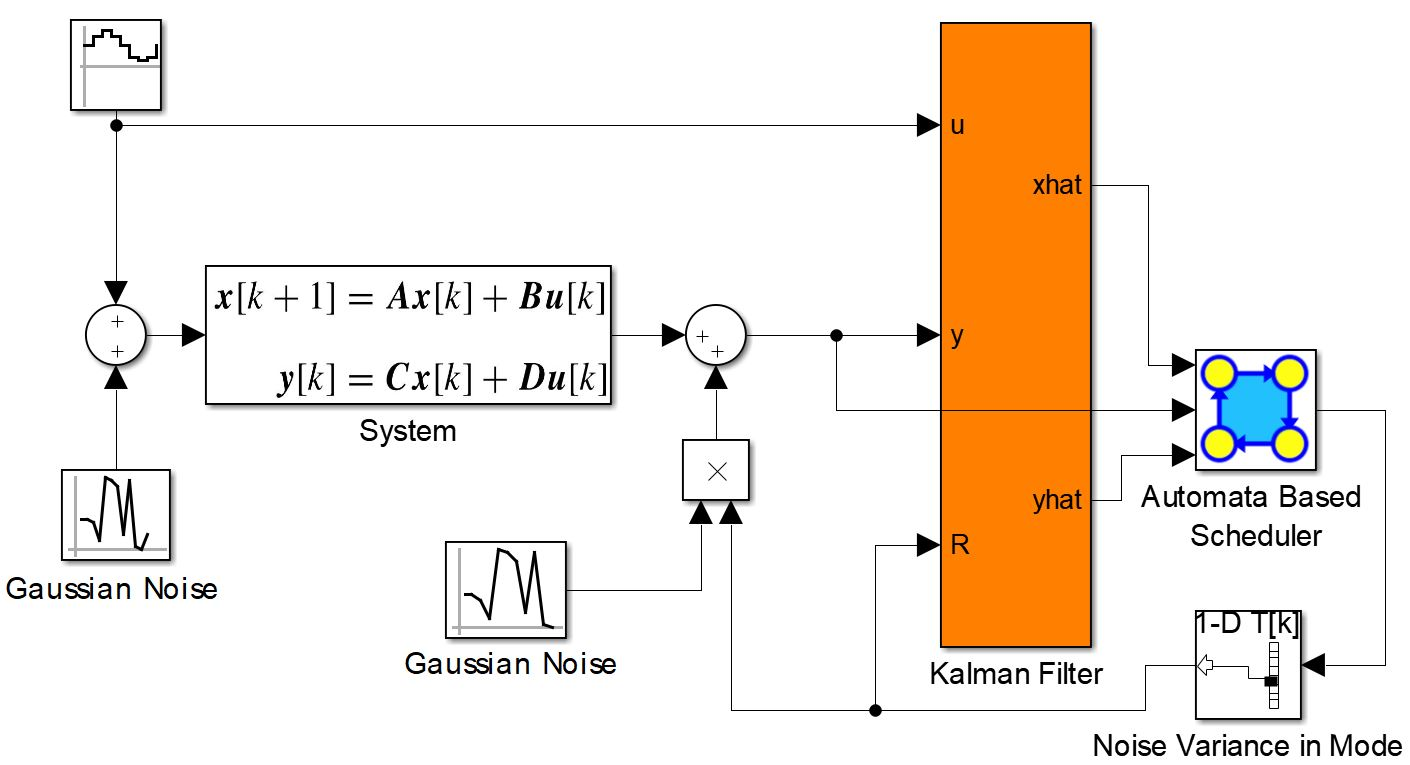
\includegraphics[width=85mm]{SimulinkModel.jpg}}
	\caption{A Simulink model demonstrating our approach.}
	\label{fig:simulink}
\end{figure}

The scheduling of the modes is governed by the automata based scheduler as depicted in Figure~\ref{fig:simulink}. We propose to use a standard Kalman filter for the purpose. The filer gets as input the actuations and the measurements (the sum of the output and the noise) and also the variance of the measurement noise, which we assume is a function of the sensor mode chosen by the scheduler. The output of the Kalman filter and the measurement are fed to the scheduler (in addition to, possibly, sending them to the controller) that uses them for deciding the next mode of the sensor. In the Simulink model depicted in Figure~\ref{fig:simulink}, the scheduler feeds the variance of the disturbance to the Kalman filter and to the block that multiplies the noise by the variance (the product of a white noise with unit variance and a constant $C$ yields a normally distributed noise with variance $C$).

We ran the model depicted in Figure~\ref{fig:simulink} with the linear time invariant system:
\begin{eqnarray*}
x(k+1) &=& \begin{pmatrix}
	1.3  & -0.5  & 0.1 \\
	1    & 0     & 0 \\
	0    & 1     & 0
\end{pmatrix}x(k)+ 
\begin{pmatrix}
-0.4 \\
0.6\\
0.5\end{pmatrix} u(k) \\
y(y)&=& \begin{pmatrix}1 & 0 &0\end{pmatrix}x(k)
\end{eqnarray*}
taken from \url{https://www.mathworks.com/help/control/examples/kalman-filter-design.html}. As seen in Figure~\ref{fig:simulink}, we injected a sinusoidal input (with $amplitude=bias=frequence=1$) to this system. 

The actuation noise, depicted on the left, is with a unit variance. The `Automata Based Scheduler' block sets the variance of the sensing noise dynamically to be either $0.25$ or $2$ at each step of the simulation. 

%A = [1.1269   -0.4940    0.1129,
%1.0000         0         0,
%0    1.0000         0];
%
%B = [-0.3832
%0.5919
%0.5191];
%
%C = [1 0 0];






%\begin{enumerate}
%    
%    \item \textbf{Controller design:} Based on the separation principle, we propose to design the controller to achieve the control objectives assuming a perfect observation. In practice, this may not be feasible because controller designs such as PID require a system to experiment with. In this case, as demonstrated in the case-study below (see Section~\ref{sec:caseStady}), we propose to work with one of the observation modes. If the system is close to linear, this should result with a near optimal design.
%    
%    \item \textbf{Observers design:} Specification of sensor modes and observers design
%    
%    \item \textbf{Performance analysis:} Now, we can perform some experiments with the different observer modes and analyze transient behaviors. Specifically, as shown in the case study~\ref{sec:caseStady_analysis}, we can measure how long it takes for the error to accumulate after switching to a lesser observation mode and formulate how this error affects the control objectives.
%
%    \item \textbf{Scheduling automata design:} Base on the analysis we can specify the resource scheduling requirements in the form of \textit{specification automaton}. The goal is to design flexible specification that allow dynamic scheduling in order to adapt the environment and the system state, this will improve the system efficient.
%
%\end{enumerate}


%\section{Application to Autonomous Quad-rotor Flying In-Door}
\section{Case Study: Stabilizing a quadrotor in front of a window}
\label{sec:caseStady}
% overview of why we use vision example

%TODO - Window test case problem
The case study we used to test our concept is the development of a controller that stabilizes a quadrotor~\cite{?} in front of a window.
We implement an autonomous controller for that task and evaluated its performance.

The part of the controller that we focused on is the vision based position controller. Specifically, the main controller, that we will describe below, uses a standard low-level angular controller and a simple image processing algorithm that identifies the position of the corners of the window in the image plane\footnote{In the experiment, to simplify the image processing algorithm, we marked the corners of the window with led lights.}. Its goal is to regulate the position of the quadrotor by tilting it. Note that rotations of the quadrotor generate a more-or-less proportional accelerations in a corresponding direction. A main challenge for this controller is that the computer vision algorithm takes significant time to compute relative to the fast control loop. We can decrease computation time by lowering the resolution, but this also increase the measurement noise. We will demonstrate how adaptive scheduling of the resolution can serve for balancing resource consumption vs. control performance.

\subsection{Observer Design}
\label{sec:Observer Design}
We first implemented an observer based on the work of Efraim at al.~\cite{?? Dynamic Image Based Visual Servo Control of Micro Aerial Vehicles Relative to a Window}. The observer gets the positions of the widow corners, enumerated clockwise starting from the top left corner noted by $p_1,p_2,p_3,p_4$, and extract 4 quantities based on the shape and location of the window corners in the image plane: $S_x$ , $s_y$ , $V_d$ and $sz$.
\textbf{center of mass:} $S_x$ and $S_y$ represent the window ``center of mass'' in the image plane along the image $x$ and $y$ axes, respectively. $S_x$ and $S_y$ are normalized to the range of $[-1,1]$.
$S_x$ is used to measure the roll angle of the window center (for stabilize the roll axis), and $S_y$ is used to measure the altitude of the drone (for stabilizing the throttle).
\textbf{Window size:} $sz$ is the sum of the vertical edges of the window, $sz$ is used to measure the distance of the drone from the window and then to regulate the roll angle~\footnote{we use fixed size window and convert $sz$ to distance (in meter in our case) based on this window, in the general case the distance is relative to the window size}.
\textbf{Vertical difference:} $V_d = \frac{y_1-y_4-(y_2-y_3)}{y_1-y_4+(y_2-y_3)}$, were $y_i$ is the vertical position of $p_i$ in the range of $[-1,1]$ (0 is the center of the image) first is used to measure the angular position of the drone in relation to the window ($\theta$), then $\theta$ and $sz$ are used to calculate the horizontal position parallel to the window surface ($x$ position) of the drone (see Figure~\ref{fig:cordinates}). 

After measuring the relative position and yaw attitude, as usual, we add estimator filter to get better state estimation. 
In theory, and s shown in the simulation at Section~\ref{sec:simulation}, we should use Kalman filter estimator for best state estimation, in our case is non-linear system and the process noise distribution is problematic to determine (battery state affects the system dynamics), this with the complexity of kalman filter lead us simplify the kalman filter principles using complementary filter, a simple estimation technique that is often used in the flight control industry.
Complementary filter is actually a steady-state Kalman filter for a certain class of filtering problems~\cite{complementaryVSKalman}.
We use two steps estimator that, (1) \textit{predict} the current state evolved from the previous state using a linearized model of the system ($\hat{x_{k|k-1}}$) and then \textit{update} the prediction with current state measurement from image explained before, noted by $z_k$.
The result estimation (noted by $\hat{x}_{k|k}$) is a complementary filter of the prediction ($\hat{x}_{k|k-1}$) and the measurement ($z_k$):
$ \hat{x}_{k|k} = K \hat{x}_{k|k-1} + (1-K) z_k $ were $K$ is constant approximation of the kalman filter gain ($K_k$).

As describe in Section~\ref{sec:???}, the image processing have few different operation modes, every mode has different accuracy.
Similarly to the gain of kalman filter, $K$ represent the ratio between process noise and measurement noise distribution, therefore $K$ is defined separately for each mode to achieve the best estimation in each mode.
For simplicity, in this work we examine only two modes, \textit{High quality} with resolution of 960p and \textit{Low quality} with resolution of 240p.

\subsection{Controller Design}

In this experiment, we consider the task of \textit{hovering in front of the window}, the controller objective is to hover parallel to the window (center of $x$ axis) at the altitude of the window within distance of 2 meters in front of the window and face pointed to the center of the window (yaw angle).
We consider this point as the origin and the coordinates are according to Fig.~\ref{fig:axis}.

\begin{figure}[htbp]
    \centerline{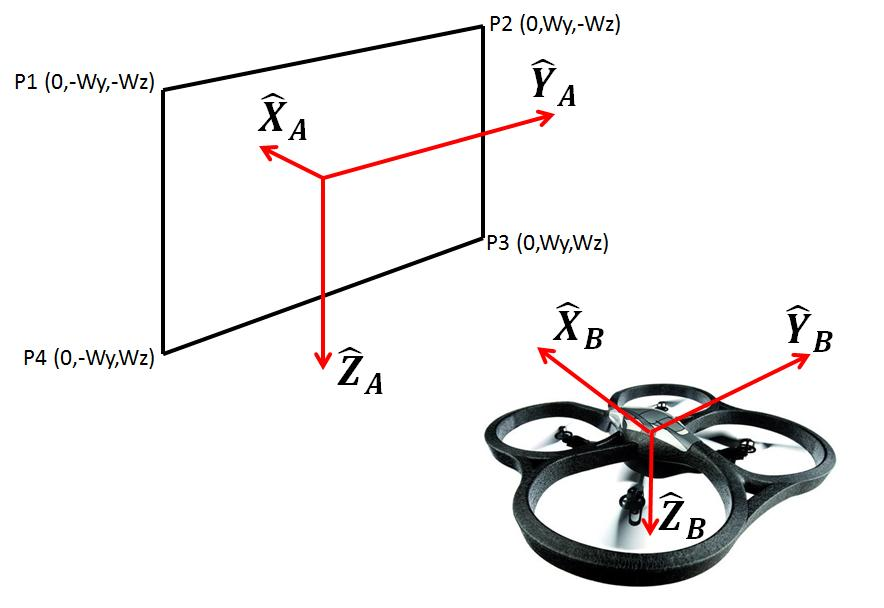
\includegraphics[width=85mm]{axes_fron_hanoch.jpg}}
    \caption{TODO fix "x" axes.}
    \label{fig:axis}
\end{figure}

The controller consist of 4 independent feedback control loops, altitude, yaw angel, pitch and roll.
Pitch and roll controllers composed from, low level attitude controller which his input is the required pitch or roll angel accordingly, and high level position controller which his input is the required distance or $x$ position relative to the window accordingly, the high level controller outputs the required angle (acceleration) to the low level controller as show in Fig.~\ref{fig:controllerStracture}.
All the loops control regulate the position or attitude relative to the window.
The inertial (angular) feedback is generated by the existing \textit{Attitude and heading reference system} (AHRS) library of ArduPilot see Section~\ref{sec:Experiment setup}, and the window related feedback come directly from the observer described in Section~\ref{sec:Observer Design}.

Based on the separation principle, we can use that controller regardless the measurement quality, in practice we implement basic Proportional Integral Derivative (PID~\cite{aastrom2006advanced}) controller and tuned the parameters with the highest resolution observer.

\begin{figure}[htbp]
    \centerline{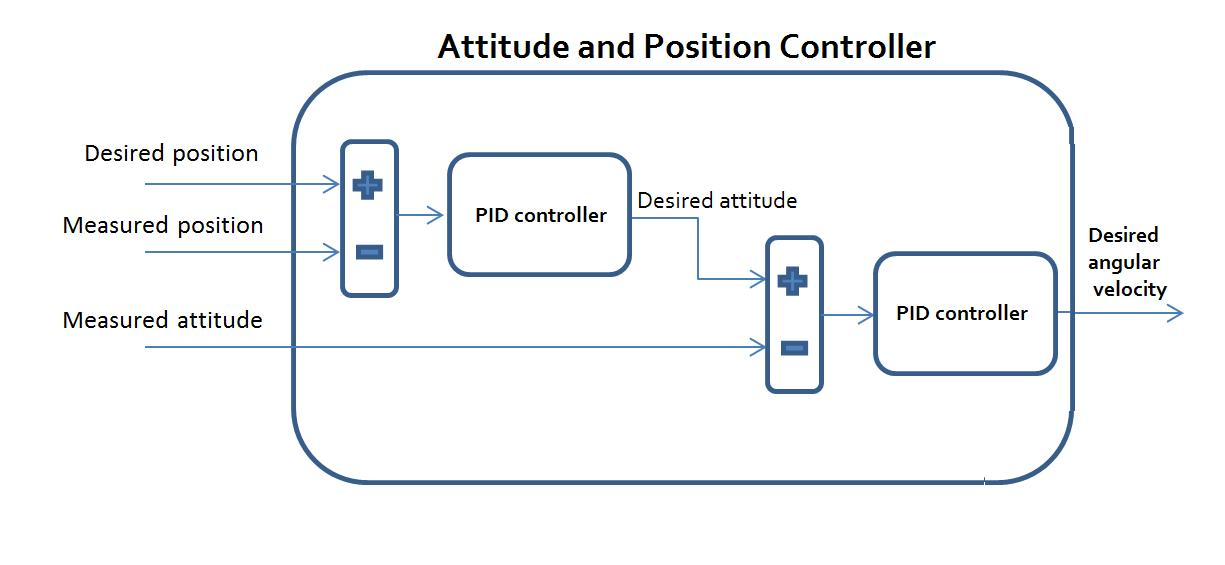
\includegraphics[width=85mm]{controller_from_hanoch.jpg}}
    \caption{TODO.}
    \label{fig:controllerStracture}
\end{figure}







%TODO - continue here
\subsection{Analysis and Specification Automata}
%As describe in Section~\ref{sec:???}, the image processing have few different operation modes, every mode use different image resolution, better image resolution results in more accurate measurement but consume more processing time, changing operation modes allows us to control the trade off between mesurment quality and processing time as shown in Table~\ref{tab:tradeoff ???}.

The objective of the system is to maintain stable hovering in front of the window. Hence, the performances of the system is measured by the amount of deviation from the center line of the window in the critical axis $x$ (see Figure~\ref{fig:axis}). Our goal is to achieve maximum performance with minimal amount of processing time, when both goals can not be achieved together we try to set the best traydoff between them. The main consumer of computation resources in this system is the image based observation tasks.

Analyzing the test results shown in Table~\ref{tab:res ???} we see that High quality observation mode provide 0.4 meter error tolerance meaning we can fly this mode in 1.2 meter wide corridor\footnote{Experiments was done with 0.4 meter wide quad-rotor}, with the cost of 30\% CPU usage. 
With adaptive scheduling specification we lower the CPU usage without significant worsening of High quality performances.

%TODO - error ($y_{k|k}$) derived schedulers
%TODO - wha realy "post-fit residual" mean??
Notation: post-fit residual $\tilde{y}_{k|k}$, is calculated as the absolute difference between the estimated state ($\hat{x}_{k|k}$) and the measured state ($z_k$): $\tilde{y}_{k|k} = |  \hat{x}_{k|k} - z_k |$.
From the Low quality experiment graph we can see that $\tilde{y}_{k|k}$ accumulates proportional to the deviation from the center of $x$ axis, we can use $\tilde{y}_{k|k}$ vales to predict high deviation from $x$.
Using simple guard automata as shown in Section~\ref{sec:scheduler} we define dynamic observer that choose the operation mode (high or low quality) based on $\tilde{y}_{k|k}$ value, as show in Fig.~\ref{fig:guard auto y_kk}, this observer operate in low quality for ``GOOD'' states, when $\tilde{y}_{k|k} < \alpha_{low}$, and change to high quality if the state is ``BAD'', when $\tilde{y}_{k|k} > \alpha_{high}$, the trash holds values $ \alpha_{low}$ and $ \alpha_{high}$ has determined first from the low and high quality graph and fine tuned by experiments. 
Different $ \alpha_{low}$ and $ \alpha_{high}$ achieve different trade-offs of performances and processing time.
Note, in Section~\ref{sec:results} we show how this dynamic observer do not result any significant affect the performance but reduce by factor of $\frac{1}{2}$ the processing time.

%TODO - displacement ($x_{k|k}$)  derived schedulers
We also examine a straight-forward solution based directly on the current position (the $x$ part of $\hat{x}_{k|k}$), we define dynamic observer similar to the $\tilde{y}_{k|k}$ based observer described above, but in this case ``GOOD'' states are states where the drone is closer to the center line of the window, and ``BAD'' states are when the drone is far.
Formally, this observer operate in low quality when $x < \alpha_x$, and in high quality when $x > \alpha_x$, this also produce similar results to the $\tilde{y}_{k|k}$ based observer.

%TODO hodai: complex / agregated schedulers (3 states) - the results shows no improvement I wont to perform new experiments with significant improvement

%TODO - gyro derived?? more suggestions?


\subsection{Results}
\label{sec:results}
TODO - graphs and tables


\begin{table}[htbp]
    \caption{Test Results}
    \begin{center}
        \begin{tabular}{m{8em} |  m{4em} m{5em} m{5em}}
        %\begin{tabular}{m{6em} |  c c c}
            \hline
            %\textbf{Observer}& CPU usage (\%)  & Mean displacement ($x$ axis) & Max displacement ($x$ axis)\\
            \textbf{Schedule}& \textbf{\% CPU}  & \textbf{mean(|$x$|) (mm)} & \textbf{max(|$x$|) (mm)}\\
            %\cline{2-3} 
            \hline
            Only High & 30.9\% & 95 & 312 \\
            \hline
            Only Low & 2.1\% & 300 & 709 \\
            \hline
            error ($y_{k|k}$) derived 10-20 & 10.3\% & 149 & 432 \\
            \hline
            error ($y_{k|k}$) derived 10-15 & 11.7\% & 113 & 363 \\
            \hline
            displacement ($x_{k|k}$) derived 10 & 16.6\% & 109 & 425 \\
            \hline
            displacement ($x_{k|k}$) derived 20 & 14.0\% & 141 & \textbf{321} \\
            \hline
            displacement ($x_{k|k}$) derived 30 & 8.9\% & 174 & \textbf{484} \\
            \hline
            4state X10-30 E10-15 & 10.4\% & 127 & 366 \\
            \hline
            3state X10 E10-15 & 8.8\% & 129 & 321 \\
            \hline
            
        \end{tabular}
        \label{tab1}
    \end{center}
\end{table}

\section{Experiment setup}
\label{sec:Experiment setup}

In order to perform the experiments we used of-the-shelf quad rotor with \textit{navio2}~\cite{navio} and \textit{Raspberry pi}~\cite{raspberry} flight controller that runs a modified \textit{ArduPilotMega-arducopter}~\cite{APM} software.
\textit{Navio2} is extension board (shield) for the \textit{Raspberry pi}~\cite{raspberry} platform, it provides the nessesary interfaces such as remote control inputs and motors output, and it's equipped with 3-axes gyroscop and accelerometer MEMS sensors~\cite{MEMS}.
%cammera
We used the standard raspberry pi camera. % and modified driver for eficient recording in 

%the window

%TODO - natnet
%TODO - vision search algorithem??

\section{Conclusions}
Conclusion goes here.


%ACKNOWLEDGMENTS are optional
\section*{Acknowledgments}
Acknowledgement goes here.


%
% The following two commands are all you need in the
% initial runs of your .tex file to
% produce the bibliography for the citations in your paper.
\bibliographystyle{abbrv}
\bibliography{reactive_scheduler}  % reactive_scheduler.bib is the name of the Bibliography in this case
% You must have a proper ".bib" file
%  and remember to run:
% latex bibtex latex latex
% to resolve all references
%
% ACM needs 'a single self-contained file'!
%
%APPENDICES are optional
%\balancecolumns
\appendix
%Appendix A

Appendix goes here.

% That's all folks!
\end{document}
